%===================================== CHAP 3 =================================

\chapter{Method} \label{chp:method}
This chapter will give an insight into why the research is needed and what method used conducting the research. Also, the chapter gives insight into the collection of data and the following analysis, as well as and who are the participants. 

This thesis is a part of two-phased research. The first phase made its results into a separate thesis: the project thesis. Data discussed in this thesis is obtained both in phase one and two. 

\section{Methodological Approach} \label{sec:purpose}
This study aims to understand the primary conditions for Norwegian construction projects, utilizing Lean and BIM, to achieve the potential of both the applied methodology and digital tools. The research is, therefore, adopting a case study-strategy of a single-case object, in the CI in Norway. Utilizing a single-case study approach, preferably than multiple, will give a more in-depth look at the problem, rather than a thin description provided by the multiple-case study \citep{yin1993case}. This research, therefore, aims to examine a case using lean methodology, utilizing digital tools to support both the method as well as cooperation and interaction between different actors. The project selected is the construction of the new Life Science Building, managed by Statsbygg \citep{statsbygg2019uio}.   

The problem of using a case study is that it is hard to produce a generalized answer to a question. The aim of the research is not to obtain generalizable findings but to explore the phenomenon. Furthermore, identify different measures that can help this specific project. This thesis is based on a preliminary project committed in the fall of 2019. The intention is not to measure productivity, but rather understand the phenomena and propose coherent actions.

This study is related to the interpretivism paradigm — the use of empirical observation of the participants and a desire to identify how they act on the new software and methods used. Using interviews can lead to being subjective as all collection of data is done in interaction with the participants. This yields a qualitative collection of data. The purpose of this master thesis is to identify issues causing a lack of productivity and identify actions fixing these issues. Moreover, implement some actions and observe how the project react to those changes. 

Due to the Covid-19 virus, this thesis could not implement the identified actions, and therefore only propose a set of actions.

\section{Access to Case}
Obtaining the LSB-project was rather by chance, and followed no formal theoretical sampling procedures proposed by the literature \citep{yin1993case}. In the fall of 2018 the researcher came in contact with Patrick Stormo Hjerpseth, former Project Manager of Digitalization in the LSB-project. After a conversation, where the researcher told about motivation and interest in methodology and software utilization, Hjerpseth came up with the idea of writing a master thesis on the LSB-project. The researcher was at the same time offered a job in Progit Consulting AS, where Hjerpseth is CEO. Moreover, signing with Progit in the fall of 2019. Hjerpseth helped gaining access to the LSB-project, and in the fall of 2019 the first phase of this research began. During the first phase of the project Hjerpseth became sick leave. Giving a new point of contact, Darre Brecke Brenden, from Statsbygg. Also, a agreement with Statsbygg was secured for the project to continue into the next phase. Which gave more access, both in terms of participants, and the posibility to use the project office doing the interviews.  

\section{Litterature review}
A literature review offering a qualitative research method and serves as an essential part of the study. A systematic search of relevant literature gives insights into different selected subjects and disciplines relevant to the research. The researcher followed no formal method in the literature review.

Utilizing google scholar as a search engine, the primary source of literature is, thus, theses, research papers, and books. Moreover, using books and literature already known to the researcher. The researcher developed a set of search words and combinations. Based on the research theme, and findings in the interviews, different combinations appeared. Search words used frequently are Lean Construction, Lean Design, Lean, Agile, BIM, CSCW, with a different combination of pre- and postfix. 

Often a set of literature was picked based on its title and thereafter minimizing the set based on the abstract and introduction. Moreover, reading the papers, the reference named is checked and evaluated. 

\section{Data Collection}
\begin{figure}
    \begin{center}
        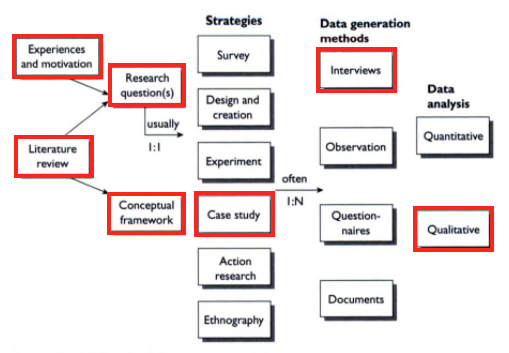
\includegraphics[width=0.75\textwidth]{fig/research_process_master.png}
        \caption{The research process used, marked with methods applied in the research.}
        \label{fig:research_process_master}
    \end{center}
\end{figure}

\subsection*{Interviews}
The interviews for this research was done during two phases, as seen in the \ref{tab:participants}. 

The first phase of the research, resulting in a project thesis, was conducted in the fall of 2019. Due to a hectic period of the project, the researcher made use of video chat conducting the interviews. Using Skype and other video chat services can be cost-effective due to the ease of planning, compared to face-to-face interviews. On the other hand, because of the small window the web camera provides, it could be challenging to read the participant's body language \citep{cater2011skype}.  Also, the utilization of digital interviews is reliant on highspeed internet, and that the subject is familiar with the digital tool for the interview to work well enough.

In the second phase, the interview took place at the project office, near the building site, in Oslo. The project gave up a small meeting room for a week for the researcher to use. Opposite of digital conduction, face-to-face interviews lead to more waste of time caused by the difficulty of planning and waiting. On the other hand, the conversation will not suffer from a lack of body language or depend on technical tools to work, but the recording device. Also, the researcher felt the conversation had a better flow face-to-face. 

On the other hand, every interview can be a source of error because of the communication element and how the actors interpret. What the interviewee sais is not only in words, but mimics, cadences, body language as well. Hence the difference in the face-to-face and video chat interviews. Using follow-up questions helps in the case of insecurity. Also, the researcher could correspond with the participants over email and telephone after the interviews. Thus, increasing the validity of the data. 

Before an interview, an email was sent to the participant, preparing for the conversation. The email consisted of a description of the research, the researcher. Moreover, the consent and interview guide described later in this section. The preparation gave the researcher more in-depth and thought-through answers. Not every participant had spent time preparing for the interview. 

The conduction of the interviews followed a set of standardized questions. The researcher, beforehand, developed these questions. The guide consists of a small collection of themes relevant to the research question, listed in Appendix \ref{apx:interview_guide}. The order in which the questions where asked was not of importance, and often changed based on the interviewee—moreover, the participant was indeed the dominant part of the interviews. The interviews are, therefore, consisting of several follow-up questions. The purpose of an unstructured interview was for the interviewee to speak freely, and therefore more receive more genuine answers. The research process used is shown in figure \ref{fig:research_process_master}.

In line with Norsk Senter for Forskningsdata AS (NSD), the researcher, signed an informed consent with the participants. The contract gives the researcher allowance to do the interview; keep personal data throughout the project, such as name, title, and company; and do recording of the interview. The purpose of the recording was for the researcher not to take heavy minutes during the interview, instead focus on the conversation. Also, a recording will give an exact version of the interview. 

The transcription became more or less the exact recording of the interview. Sometimes, not writing the follow-up questions, if the sentence made sense. The resulting text was hard to read, due to its spoken tone of voice. The purpose was not to make a perfectly readable text, but to have documentation of the thoughts and experience of the subjects, for further analysis. Moreover, after the interview, the transcript was sent to the participants for them to approve. Every interview lasted between 15 minutes and up to half an hour.

\subsection*{Observations}
This research has, in addition to interviews, as one can see from figure \ref{fig:research_process_master}, utilized observations to obtain information and data. Moreover, the research has used a set of documents describing the project, project vision, and strategy. 

The observations took place over the first phase of the research. During two days at the project office, observing different meetings, the researcher recorded with notes what was happening and said in the meetings, and transcribed after the fact. The list of observations is placed in table \ref{tab:observations}. 

\begin{table}
    \begin{center}
        \begin{tabular}{p{.45\textwidth}p{.45\textwidth}}
        \toprule
        \textbf{Obervation} & \textbf{Meeting}              \\ \midrule
        1                   & Blackboard-meeting            \\
        2                   & Table-test meeting            \\
        3                   & Digitalization-meeting        \\
        4                   & BIM and dRofus introduction   \\
        5                   & Being in the Project office   \\
        Total observations  & \multicolumn{1}{r}{5}  \\ \bottomrule
        \end{tabular}
        \caption{List of observations conducted in the project thesis.}
        \label{tab:observations}
    \end{center}
\end{table}

The transcription of the records was to write out the notes written during the observations. Besides, writing down questions and thoughts connected to obtained literature. Except for the Digitalization meeting, the researcher was not able to ask questions during the meeting. Questions who came up was later answered by managers, or directly with participants, after the meetings. In addition to the observations and answering questions, talking to the managers and PLs, on-site, gave valuable insight into the project.

\subsection*{Documents}
Documents were vital in gaining insight into the project. Statsbygg, as the manager, documents the construction in \citep{statsbygg2019uio}. Moreover, UiO, as the final user of the building, gave valuable documentation of the construction and the final building, used in describing the construction \citep{uio2019science}. Also, documentation of the prior constructed Bergen Academy of Art and Design \citep{lean_i_praksis} gave valuable insight into how the manager planned for the LSB-construction. Moreover, propose the overall strategy used in the LSB-project, described in section \ref{sec:strategy}. Besides, giving birth to the ide behind the Cogito Project resulting in the tool used. 

\section{Participants}
The project researcher, Morten Bujordet, is involved in the project, creating the plans, and conducting the research.
	 
Supervising the project is Eric Monteiro. Monteiro is contributing with experience in research in the implementation and use of new digital tools in large scale, as welle as complex organizations. 

Furthermore, Statsbygg, as the manager, has an interest in the project: giving access to the participants in the study. With Darre Brecke Brenden as the point of contact.
	 
In the research, the actors in all layers and disciplines of the project organization will be an aim for the data collection. The thesis conducted a total of 18 interviews. Selecting the first two interview objects was based on a list of 6 interviewees, proposed by the first contact person. Only two subjects had the opportunity to participate, due to a hectic period of the project.  The second phase of interviews started with a list of 32 potential interview objects. Every proposed interviewee was contacted; only 16 had the opportunity. The initial list of persons was handpicked, by the assisting project director, to get an insight into all different levels of seniority and different disciplines of the project. The resulting set of interviews represent a wide range of project seniority. From a month of experience and up to the very start of the project, back in 2014. Also, the set represents every discipline in the project. The interviewees are listed in table \ref{tab:participants}.

All personal information gathered will, safely, be stored in a GDPR-compliant Cloud Service, served by NTNU. In the final report, no personal information will be published, and all participants will be anonymized.


\begin{table}
    \resizebox{\textwidth}{!}{%
    \begin{tabular}{@{}lllll@{}}
    \toprule
    \textbf{Interviewee} & \textbf{Function} & \textbf{Gender} & \textbf{\begin{tabular}[c]{@{}l@{}}Phase 1\\ (November 2019)\end{tabular}} & \textbf{\begin{tabular}[c]{@{}l@{}}Phase 2\\ (February 2020)\end{tabular}} \\ \midrule
        1 & \begin{tabular}[c]{@{}l@{}}Assistant Project Director \& \\ Project Manager \end{tabular} & Male & x & \\
        2 & Assistant Project Manager  & Male & x & \\ 
        3 & Project Manager & Male & & x \\
        4 & Engineering Manager & Male & & x \\
        5 & Engineering Manager & Male & & x \\
        6 & Progress Planner & Female & & x \\
        7 & ITB Manager & Male & & x \\
        8 & Associate & Female & & x \\
        9 & Discipline Leader & Male & & x \\
        10 & Discipline Leader & Female & & x \\
        11 & BIM Manager & Male & & x \\
        12 & Associate & Male & & x \\
        13 & Associate & Male & & x \\
        14 & Discipline Leader & Male & & x \\
        15 & Assiciate & Male & & x \\
        16 & Ass. Project Group Leader & Female & & x \\
        17 & Engineering Manager & Male & & x \\
        18 & BIM Coordinator & Male & & x \\
        Total interviews & \multicolumn{2}{r}{} & 2 & 16 = 18\\ \bottomrule
    \end{tabular}%
    }
    \caption{Overview of interviews and phases of data collection.}
    \label{tab:participants}
\end{table}

\section{Data Analysis}
The analysis started by transcribing the interviews and sent to the participants for approval. Furthermore, utilizing a thematic analysis approach. The thematic analysis followed a set of steps

\begin{enumerate}
    \item { \bf Perusal of all the material:} It was essential to get to know the material, and read through all the interviews. The interviews were already familiar because of listening to the recordings when transcribing and conducting the interviews. Reading through the interviews gave a more in-depth understanding. Moreover, it allowed the researcher to reflect on the answers with the preliminary literature review.; 
    \item { \bf Generation of codes}: After getting to know the material it the focus was to identify parts of the text based on the project question, marked with an identifying code. The focus of the coding was identifying text of interest, based on the literature review, the researcher's technical view, and the research question. Every code is an attempt of generalization of the corresponding text. When logging the codes, the code itself, a snippet of the corresponding text, and the context the sentence appeared was listed in a excel sheet. After coding, the researcher changed the naming of some codes which had a relation or the same meaning. Making the collection of themes easier; 
    \item { \bf Collection of themes}: Based on the codes, a set of themes evolved. The codes find most connected were put into groups, based on the connection between them. Utilizing mind map grouping the different themes. Drafting different groupings, based on themes and relevant literature; 
    \item  { \bf Reviewing the themes}: The researcher wrote a list of potential discussions and findings for each of the five collected themes. The literature review, polarizing answers, and the technical level of the theme made the basis of the collected themes. Also, the researcher's considerations made for the final choice of themes; 
    \item { \bf Defining and naming the themes}: The previous step resulted in two themes for this step to name. From here, every code, every theme, every interview was written in Norwegian. The first iteration of naming was, therefore, a direct translation of the theme and, thus, not well articulated. The resulting themes are: (1) Overlapping software functionality and software usage, (2) Lack of fundamental methodological knowledge;
    \item { \bf Producing the report:} Describing the findings in the thematic analysis, using the chosen themes as a guideline. Moreover, discussing the themes with relevant literature, previous experience, and context.
\end{enumerate}

The data produced in this process is in the Appendix. The initial codes identified Appendix \ref{apx:codes}. The collection of themes and eviewing of themes did not produce much data, due to its subjective manifestation. 

\begin{table}[]
    \centering
    \begin{tabular}{p{0.2\textwidth}p{0.32\textwidth}p{0.19\textwidth}l}
    \toprule
    \textbf{Code}           & \textbf{Excerpt of the Quote}                      & \textbf{Context/theme}      & \textbf{Participant} \\ \midrule
    Communication in BIM    & \textit{"There you talk and discuss on a reasonable basis"} & Collaborate across - BIM    & ITB Manager          \\
    Communication in Cogito & \textit{"...but you lack the communication element"}        & Collaborate across - Cogito & ITB Manager          \\ \bottomrule
    \end{tabular}
    \caption{Two example codes from the thematic analysis}
    \label{tab:code-example}
\end{table}

After the initial step of \textit{perusal of all material}, the researcher started the generation of codes. Identifying the two codes, listed in table \ref{tab:code-example}, was identified because of the mention of two essential software and processes used in project collaboration. In both cases, the codes have the origin in the second phase of the interviews. Moreover, the attention of BIM came from the first phase, and later in the inspection of literature, accepting BIM as essential groupware in a construction process. In the case of Cogito, the first phase of the project argued for further investigation in the tool, hence why the generation of the code.

Furthermore, the \textit{excerpt of the quote} gave a context, later used in the collection and review of themes. In the case of BIM, the resulting theme did not end up in the defining of the final two hemes. Moreover, it gave valuable data for the later discussion. The Cogito code, on the other hand, was used in the final theme \ref{sec:unmitigated}; Describing the reason for the case. Moreover, alongside other codes in the theme, adding to the later discussion. 

\section{Evaluation of the Method}
The single-case study, as well as the use of unstructured interviews, produce results that cannot be generalized beyond the sample group. Still, they provide a more in-depth understanding of participants’ perceptions, motivations, and emotions. 

One can always argue that utilizing interviews for data collection can tend to be subjective. However, the use of a qualitative approach is best when wanting to describe, contextualize, and gain an in-depth insight into specific concepts or phenomena, which was the case in this empirical study. Furthermore, the project researcher has a part-time job developing the Cogito tool, which can argue for the researcher for being subjective. Though, in this case, 14 of 16 participants mentions Cogito, without the researcher asking them. Also, the participants did not know the relation the researcher had to Cogito; thus, the interviewees spoke freely. Moreover, based on the interviews, the Cogito tool was the one subject getting the most tension; therefore, discussing Cogito and themes related is arguably based on a valid reason. 

The objective of this thesis was to test some of the concluding proposals and observe the change it might bring. Though, due to the Covid-19 virus, the implementation phase was not feasible. Thus, this thesis only consists of a set of proposed actions. Testing of the actions is, therefore, up to a later project, or for the LSB-project to do. The project owner has received a summary of this research, including the proposed actions. 

Further exploration of the project question is needed to conclude on the matter, moreover, testing of the suggested actions.
\cleardoublepage